\documentclass[11pt]{article}
\usepackage[margin=1in]{geometry}
\usepackage{amsmath,amssymb,amsthm}
\usepackage{mathtools}
\usepackage{microtype}
\usepackage{graphicx}
\usepackage{booktabs}
\usepackage[section]{placeins}
\usepackage{xcolor}
\usepackage[hidelinks]{hyperref}
\usepackage[capitalise,nameinlink]{cleveref}

\graphicspath{{figures/}}

\newtheorem{proposition}{Proposition}
\newtheorem{corollary}{Corollary}
\theoremstyle{definition}
\newtheorem{definition}{Definition}

\newcommand{\Bone}{B_1^{+}}
\newcommand{\Tone}{T_1}
\newcommand{\Ttwo}{T_2}
\newcommand{\Ttwos}{T_2^{*}}
\newcommand{\Mzero}{M_0}
\newcommand{\TR}{T_R}
\newcommand{\dw}{\Delta\omega}
\newcommand{\E}{\mathrm{e}}
\newcommand{\Fi}{\mathcal{I}}
\renewcommand{\Re}{\operatorname{Re}}
\newcommand{\sgn}{\operatorname{sign}}

\newcommand{\AliasNone}{8\,697}
\newcommand{\AliasMagnitude}{42\,293}
\newcommand{\AliasComplex}{94\,540}


\title{Choosing the two flip angles of an MPME protocol:\\
an optimal-design study\\[4pt]
\large Technical note}
\author{Sarang Joshi}
\date{\today}

\begin{document}
\maketitle

\begin{abstract}
The multi-pathway multi-echo (MPME) protocol of Cheng et al.~\cite{cheng2019} acquires two
steady-state scans that differ only in the flip angle ($15^\circ$ and $330^\circ$). We ask which pair of flip
angles best determines $\Tone$ and the other parameters. Using the Ernst-angle form of the
signal invariants, we show that each scan reports only the offset of its flip angle from the
tissue's Ernst angle, that the information of a design is the sum of two single-scan
informations, and that two scans determine $\Bone$ through a lever $c(x_2)-c(x_1)$, $c(x)=x/\sin x$. This
gives exact closed-form Cram\'er--Rao bounds and a closed-form bias for pulse-ratio errors. An
exhaustive search over 145\,530 pairs, the transmit range $\Bone\in[0.7,1.3]$ and five tissues, with an
analytic check for exact aliases, finds a flat optimum that contains the published design: no
choice of angles improves the mean $\Tone$ bound by more than $2\%$ or the worst case by more than $3.2\%$.
The angles matter instead for robustness. Unmodelled finite pulses and flip-angle spreads bias
$\Tone$ most where the scan-2 pulse approaches $360^\circ$. A second pulse near $270^\circ$, which keeps that crossing
out of the $\Bone$ range, nearly halves the worst-case $\Bone$ bound, needs $30$--$33\%$ less energy at equal
pulse duration, has no aliases when fitted within its crossing-free range, and at $\Bone=1$ is nine times
less biased in WM and GM by unmodelled finite pulses of the same peak $\Bone$ (but not at the top of the $\Bone$
range), at a $3$--$7\%$ cost in mean $\Tone$ precision. Every design transfers a pulse-ratio error to $\Tone$ with
a factor of at least $1.6$, and every design should model its finite pulses.
\end{abstract}

\section*{Summary of findings}

\begin{enumerate}
\item \textbf{Structure (\cref{sec:theory}).} A design's information is $\Fi_1(\Bone\alpha_1)+\Fi_1(\Bone\alpha_2)$. Per
  scan, the $\Tone$ column of the Jacobian is $h(J_{\Bone}/c-J_{\Mzero})$, so a scan sees $\Bone$ and $\Tone$ only through
  its offset from the Ernst angle. Pulses with equal $|\tan(x/2)|$ (e.g.\ $30^\circ$ and $330^\circ$) carry the same
  per-scan information and differ only in the rate $c(x)=x/\sin x$ at which they move with $\Bone$ ($1.05$
  and $-11.5$).
\item \textbf{Closed forms (\cref{prop:closed,prop:ratio}).} $\mathrm{SD}(\ln\Bone)$ is the SD of the difference of
  the two offsets divided by the lever $L=c_2-c_1$, and $\mathrm{SD}(\ln\Tone)$ that of a lever-weighted
  combination; the $\Bone$ uncertainty reaches $\Tone$ with the factor $c_1/h\approx2$. A pulse-ratio error $\varepsilon$ gives
  $\delta\ln\Tone=-c_1c_2\varepsilon/(hL)$, $|\delta\ln\Tone|\ge1.64\,\varepsilon$, with zero residual.
\item \textbf{Flat optimum (\cref{sec:maps}).} Best mean $\Tone$ bound $49.2$ at $14^\circ/309^\circ$ (published: $50.2$);
  best worst case $100.3$ at $20^\circ/276^\circ$ (published: $103.6$). The $5\%$ band extends over $\alpha_1=11$--$20^\circ$,
  $\alpha_2=267$--$348^\circ$.
\item \textbf{The $360^\circ$ crossing.} Where $\Bone\alpha_2=360^\circ$ scan 2 measures only $\Bone$; the $\Tone$ bound peaks there
  ($0.5\%$ wide in $\Bone$ for CSF, $1$--$1.3\%$ for parenchyma), and this peak decides the worst case.
\item \textbf{Aliases (\cref{sec:aliases}).} Exact aliases are the other roots of
  $\tan(\Bone\alpha_2/2)/\tan(\Bone\alpha_1/2)=\xi_2/\xi_1$ and depend on $\Bone$ alone; $\mathrm d\ln|f|/\mathrm d\ln\Bone$ equals the lever. A
  design whose pulses stay within $(0^\circ,180^\circ)$ and $(180^\circ,360^\circ)$ over the fitting range has none.
\item \textbf{Constraints (\cref{sec:constraints}).} Pulses above $\approx300^\circ$ buy nothing; limiting the largest
  angle to $240^\circ$ costs $6$--$14\%$, to $180^\circ$ $25$--$52\%$. For the two-stage pipeline $\alpha_1=17$--$19^\circ$ is best.
\item \textbf{Model error (\cref{sec:robustness}).} Unmodelled finite pulses (equal peak $\Bone$, $1$\,ms for $330^\circ$)
  bias $\Tone$ by $10$--$20\%$ wherever the scan-2 angle passes $330$--$350^\circ$ ($20\%$ at $\Bone=1$ with $330^\circ$, $2\%$ with
  $270^\circ$); slab-edge flip-angle spreads near or across $360^\circ$ bias $\Tone$ by $13$--$74\%$. On resonance both are
  often hard to detect. Recommendation (\cref{sec:recommendations}): $\alpha_1\approx17$--$21^\circ$,
  $\alpha_2\approx255$--$270^\circ$ for $\Bone\le1.3$, finite pulses in the model, a calibrated pulse ratio.
\end{enumerate}

\section{Setting and design problem}\label{sec:setting}

\subsection{The model in brief}

The MPME sequence~\cite{cheng2019} is an unbalanced steady-state gradient echo that records
three configuration pathways ($k=+1,0,-1$), three echoes each, in each of two scans. The two
scans share the repetition time $\TR=25$\,ms and the readout and differ only in the nominal flip
angle; the actual angle of scan $i$ is $x_i=\Bone\alpha_i$. The unknowns are
$\theta=(\ln\Mzero,\ln\Bone,\ln\Tone,\ln\Ttwo,\ln\Ttwos,\dw,\phi_0)$, with logarithms for the positive
parameters so that standard deviations are relative. We use the following results of the
companion technical note~\cite{technote}.

\begin{itemize}
\item \emph{Two invariants per scan.} Each pathway amplitude is $a_k=v\,G_k(u,E_2,\dw)$, where
  $u$ and $v$ depend on the flip angle and $\Tone$ only, and $G_k$ does not depend on either.
\item \emph{Ernst-angle form.} With the Ernst angle $\alpha_E=\arccos\E^{-\TR/\Tone}$ and
  $\zeta=\tan(\alpha_E/2)=\sqrt{\tanh(\TR/2\Tone)}$, define the \emph{offset} of a sample from the Ernst angle
  \begin{equation}
    w=\ln|\tan(x/2)|-\ln\zeta .
    \label{eq:w}
  \end{equation}
  Then $u=\tanh w$ and $|v|=\zeta\operatorname{sech}w$, with $\sgn v=\sgn\tan(x/2)$. On the axis
  $s=\ln|\tan(x/2)|$ the spoiled-gradient-echo amplitude is a $\operatorname{sech}$ bump centred at the
  Ernst angle; a scan samples it at $s$.
\item \emph{What the data determine.} After the echo decay and phases have fixed $\Ttwo$, $\Ttwos$,
  $\dw$ and $\phi_0$, one scan determines its offset $w$ and the amplitude $\ell=\ln(\Mzero\zeta)$; two
  scans determine $w_1$, $w_2$ and the shared $\ell$, three numbers for $(\Mzero,\Bone,\Tone)$. One scan
  alone cannot determine $\Bone$.
\end{itemize}

\subsection{The design problem}\label{sec:problem}

\paragraph{Design variables.} The nominal angles $0<\alpha_1<\alpha_2\le540^\circ$; $\TR$ and the
readout are fixed, so every design has the same acquisition time.

\paragraph{Criterion.} The Cram\'er--Rao bound (CRLB) on $\ln\Tone$ with all seven parameters free,
in units of $\sigma/\Mzero$ (complex Gaussian noise, standard deviation $\sigma$ per real and
imaginary part). Bounds on $\ln\Bone$, $\ln\Ttwo$ and $\ln\Mzero$ are reported alongside.

\paragraph{Robustness range.} The design must work for every $\Bone\in[0.7,1.3]$ (the brain at
3\,T, central to peripheral) and the five tissues of \cref{tab:tissues}. We report the
\emph{worst case} of the bound over this range and its \emph{mean} (uniform over $\Bone$, equal
weight per tissue).

\begin{table}[!htbp]
\centering
\caption{Tissues of the robustness range ($\Mzero=1$ for all, so bounds are relative to each
tissue's own signal). Ernst angles at $\TR=25$\,ms.}
\label{tab:tissues}
\small
\begin{tabular}{lcccc}
\toprule
Tissue & $\Tone$ (ms) & $\Ttwo$ (ms) & $\Ttwos$ (ms) & $\alpha_E$ ($^\circ$)\\
\midrule
CSF & 4000 & 1500 & 900 & 6.4\\
grey matter (GM) & 1350 & 90 & 60 & 11.0\\
white matter (WM) & 850 & 66 & 50 & 13.8\\
deep GM & 1130 & 58 & 40 & 12.0\\
lesion & 1500 & 120 & 80 & 10.4\\
\bottomrule
\end{tabular}
\end{table}

\paragraph{Pipelines.} Two uses of the data lead to different optima.
\begin{itemize}
\item \emph{Joint fit}: both scans at full resolution, all parameters fitted per voxel; the
  criterion is the joint $\Tone$ bound above.
\item \emph{Two-stage}: a short, low-resolution scan 2 gives a smooth $\Bone$ map whose noise is
  negligible after smoothing~\cite[Sec.~5]{technote}, and $\Tone$ comes from scan 1 with $\Bone$
  known. The criterion for $\alpha_1$ is the scan-1 $\Tone$ bound with $\Bone$ known; $\alpha_2$ only needs to
  determine $\Bone$ reliably.
\end{itemize}

\paragraph{Constraints.} The scans are acquired one after the other, so the specific absorption
rate (SAR) of each scan scales as the square of its own angle for a fixed pulse, and a
peak-$\Bone$ limit fixes the shortest duration of the largest pulse. Both constrain the largest
angle $\alpha_{\max}=\alpha_2$; we report the best design as a function of $\alpha_{\max}$.

\paragraph{Identifiability.} A design must not admit a complex alias (\cref{def:alias}) for any true
$\Bone$ in the robustness range within the fitting range $\Bone\in[0.6,1.4]$; this is checked analytically
(\cref{sec:aliases}). Magnitude aliases are allowed: complex data, the FID-sign test or, for some
designs, a narrower fitting range remove them.

\paragraph{Model error.} Finally, the shortlisted designs are compared for their bias under
errors the fitting model ignores: a pulse-ratio error, finite pulse duration, slice or slab
profile (\cref{sec:robustness}).

\section{Theory: what a pair of flip angles buys}\label{sec:theory}

Write $c(x)=x/\sin x$ ($x$ in radians) and $h=\tau/(2\sinh\tau)$ with $\tau=\TR/\Tone$; $h\approx1/2$ for
$\Tone\gg\TR$.

\begin{proposition}[Decomposition]\label{prop:decomp}
The Fisher information of a two-scan design at transmit scale $\Bone$ is
\begin{equation}
  \Fi(\alpha_1,\alpha_2;\Bone)=\Fi_1(\Bone\alpha_1)+\Fi_1(\Bone\alpha_2),
  \label{eq:decomp}
\end{equation}
where $\Fi_1(x)$ is the information of a single scan at actual flip angle $x$, and the $\ln\Bone$
column of a single-scan Jacobian is $\partial/\partial\ln x$.
\end{proposition}
\begin{proof}
The scans have independent noise, so their informations add. Within one scan $\Bone$ enters only
through $x=\Bone\alpha$, so $\partial/\partial\ln\Bone=x\,\partial/\partial x=\partial/\partial\ln x$.
\end{proof}

\Cref{prop:decomp} makes an exhaustive search cheap: $\Fi_1$ is tabulated once per tissue on the
actual angles that occur, and every design at every $\Bone$ is a sum of two $7\times7$ matrices. It
agrees with direct evaluation of the two-scan information to $3\times10^{-15}$.

\begin{proposition}[One scan in Ernst-angle coordinates]\label{prop:perscan}
Fix $\Ttwo$, $\Ttwos$, $\dw$, $\phi_0$. The signal of one scan depends on $(\Mzero,\Bone,\Tone)$ only through
the offset $w$ of \eqref{eq:w} and $\ell=\ln(\Mzero\zeta)$, with
\begin{equation}
  \frac{\partial w}{\partial\ln\Bone}=c(x),\qquad\frac{\partial w}{\partial\ln\Tone}=h,\qquad
  \frac{\partial\ell}{\partial\ln\Tone}=-h,\qquad\frac{\partial\ell}{\partial\ln\Mzero}=1 .
  \label{eq:chain}
\end{equation}
Consequently its Jacobian columns satisfy $J_{\Tone}=h\,(J_{\Bone}/c-J_{\Mzero})$, and its information about
$(w,\ell)$ depends on the flip angle only through $w$ (for given $\ell$, $\Ttwo$, $\Ttwos$, $\dw$). Angles with equal
$|\tan(x/2)|$, i.e.\ $x$ and $\pm x+360^\circ m$, therefore carry the same information and differ only in the
rate $c$: $\Fi_1(x')=D\,\Fi_1(x)\,D$, where $D$ multiplies the $\ln\Bone$ row and column by $c(x')/c(x)$.
\end{proposition}
\begin{proof}
By the two-invariant form and the Ernst-angle form,
\[
  \Mzero a_k=\sgn\bigl(\tan\tfrac x2\bigr)\,\E^\ell\operatorname{sech}(w)\,G_k(\tanh w,E_2,\dw),
\]
which depends on $(\Mzero,\Bone,\Tone)$ through $(w,\ell)$ only; the sign is constant between multiples
of $180^\circ$ (it changes sign there, which is what produces aliases, \cref{sec:aliases}) and does not
enter the information.
The derivatives follow from $\zeta^2=\tanh(\tau/2)$ and
\[
  \frac{\mathrm d\ln|\tan(x/2)|}{\mathrm d\ln x}=\frac{x}{\sin x}=c,\qquad
  \frac{\mathrm d\ln\zeta}{\mathrm d\ln\tau}=\frac{\tau}{2\sinh\tau}=h,\qquad
  \frac{\mathrm d\ln\tau}{\mathrm d\ln\Tone}=-1 .
\] The information about $(w,\ell)$ is $\Re$ of the Gram matrix of
$(\partial S/\partial w,\partial S/\partial\ell)$, a function of $w$ alone.
\end{proof}

The identity $J_{\Tone}=h(J_{\Bone}/c-J_{\Mzero})$ holds numerically to $10^{-14}$ at the angles tested. It is the
precise sense in which a single scan cannot separate $\Bone$ from $\Tone$: the $\Tone$ column is a fixed
combination of the other two. It also says that a $330^\circ$ pulse is a $30^\circ$ pulse ($|\tan165^\circ|=
\tan15^\circ$) whose sample moves eleven times faster with $\Bone$, and in the opposite direction (we call
$c(x)$ the \emph{rate} of a scan):
$c(30^\circ)=1.05$, $c(330^\circ)=-11.5$ (\cref{fig:theory}a,b). The per-scan information on $w$
(\cref{fig:theory}c) peaks a little above the Ernst angle for the parenchymal tissues
($w=0.1$--$0.4$, actual angles $13$--$16^\circ$) and well above it for CSF ($w=1.85$, $39^\circ$), whose long $\Ttwo$
makes the pathway ratios informative at larger angles.

\begin{proposition}[Two scans: closed-form bounds]\label{prop:closed}
Let $L=c(x_2)-c(x_1)\ne0$ be the \emph{lever} of the design (the difference of the per-scan rates
$c$), and let $Q$ be the information about $(w_1,w_2)$ after the
shared amplitude $\ell$ and the parameters $\ln\Ttwo$, $\ln\Ttwos$, $\dw$, $\phi_0$ have been profiled out. Then the
Cram\'er--Rao bounds of the full model are
\begin{align}
  \mathrm{SD}(\ln\Bone)&=\frac{\sqrt{e^{\mathsf T}Q^{-1}e}}{|L|},\quad e=(-1,1),&
  \mathrm{SD}(\ln\Tone)&=\frac{\sqrt{g^{\mathsf T}Q^{-1}g}}{h\,|L|},\quad g=(c_2,-c_1),
  \label{eq:closed}
\end{align}
and with $\Bone$ known $\mathrm{SD}(\ln\Tone)=1/(h\sqrt{\mathbf 1^{\mathsf T}Q\mathbf 1})$. With $\Ttwo$, $\Ttwos$, $\dw$, $\phi_0$ known, the
same formulas hold with $Q$ profiled over $\ell$ only.
\end{proposition}
\begin{proof}
By \eqref{eq:chain}, the map $\theta\mapsto(w_1,w_2,\ell,\ln\Ttwo,\ln\Ttwos,\dw,\phi_0)$ is a local diffeomorphism whose
Jacobian has the block $\begin{psmallmatrix}0&c_1&h\\0&c_2&h\\1&0&-h\end{psmallmatrix}$ in $(\ln\Mzero,\ln\Bone,\ln\Tone)$, of
determinant $-hL$, and the identity in the remaining parameters. Inverting it, to first order
$\mathrm d\ln\Bone=(\mathrm dw_2-\mathrm dw_1)/L$ and $h\,\mathrm d\ln\Tone=(c_2\,\mathrm dw_1-c_1\,\mathrm dw_2)/L$. The bounds transform with the
Jacobian, so the covariance of $(\ln\Bone,\ln\Tone)$ is that of $(w_1,w_2)$, i.e.\ $Q^{-1}$ (the inverse of
the information profiled over all other coordinates), mapped by these two linear forms. With
$\Bone$ known, $\mathrm dw_1=\mathrm dw_2=h\,\mathrm d\ln\Tone$, so the information about $h\ln\Tone$ is $\mathbf1^{\mathsf T}Q\mathbf1$.
\end{proof}

\Cref{prop:closed} separates the design into two ingredients: \emph{where} each scan samples the
bump (through $Q$, which depends on the offsets $w_1$, $w_2$) and \emph{how differently} the two samples
move with $\Bone$ (through $L$). $\Bone$ is measured by the difference of the offsets divided by the lever,
$\Tone$ by a lever-weighted combination. Writing $g=L\,e_1-c_1e$ with $e_1=(1,0)$ gives the exact decomposition
\begin{equation}
  \mathrm{Var}(\ln\Tone)=\frac{(Q^{-1})_{11}+2(c_1/L)\bigl[(Q^{-1})_{11}-(Q^{-1})_{12}\bigr]}{h^2}
  +\Bigl(\frac{c_1}{h}\Bigr)^2\mathrm{Var}(\ln\Bone):
  \label{eq:t1decomp}
\end{equation}
the $\Tone$ uncertainty is a scan-1 term plus the $\Bone$ uncertainty carried over with the factor
$c_1/h\approx2c_1$, the same factor that carries a pulse-ratio error (\cref{prop:ratio}). Three
consequences follow.

\begin{itemize}
\item \emph{Large levers.} As $|L|$ grows, $\mathrm{Var}(\ln\Tone)\to(Q^{-1})_{11}/h^2+(c_1/h)^2\mathrm{Var}(\ln\Bone)$, with a correction of
  order $c_1/L$. For the published design ($L=-12.5$) the correction lowers the variance by about a
  fifth (WM: from $937$ to $746$); for $|L|\approx6$, as in the no-crossing designs, it is comparable to the
  total, and the limit is not a useful approximation. The lever is
  largest where $\sin x_2\to0$, i.e.\ at $x_2=180^\circ m$, but there the scan-2 signal vanishes too. At such a
  crossing \cref{prop:closed} holds only as a limit; directly, the scan-2 Jacobian then has a
  single non-zero column, $\ln\Bone$ (the signal is zero but its derivative is not), so scan 2 measures
  $\Bone$ alone, a null measurement. Because the single-scan null direction
  $(\delta\ln\Mzero,\delta\ln\Bone,\delta\ln\Tone)\propto(h,-h/c_1,1)$ has a non-zero $\Bone$ component, the information matrix stays
  non-singular (the bounds finite) unless $x_1$ is also at a crossing.
\item \emph{Small angles.} For two small angles $c_1\approx c_2\approx1$, $L\to0$, and both bounds diverge:
  the leading-order degeneracy of small-angle protocols~\cite{technote}.
\item \emph{Equivalent pulses.} $30^\circ$, $330^\circ$, $390^\circ$ and $690^\circ$ have the same per-scan information
  but rates $c=1.05$, $-11.5$, $13.6$ and $-24.1$. A larger rate helps only if the pulse does not
  cross a multiple of $180^\circ$ over the range of $\Bone$ and is affordable in SAR.
\end{itemize}

\begin{proposition}[Pulse-ratio error]\label{prop:ratio}
Suppose the actual scan-2 angle is $(1+\varepsilon)$ times its nominal value relative to scan 1 and the
fit assumes the nominal ratio. Then, to first order and whichever of $\Ttwo$, $\Ttwos$, $\dw$, $\phi_0$ are
fitted,
\begin{equation}
  \delta\ln\Tone=-\frac{c_1c_2}{h\,L}\,\varepsilon,\qquad \delta\ln\Bone=\frac{c_2}{L}\,\varepsilon,\qquad
  \delta\ln\Mzero=h\,\delta\ln\Tone ,
  \label{eq:ratiobias}
\end{equation}
$\Ttwo$, $\Ttwos$, $\dw$, $\phi_0$ are unbiased, and the fit has zero residual: the error cannot be detected
from the data.
\end{proposition}
\begin{proof}
The error shifts the scan-2 offset by $c_2\varepsilon$ and nothing else, so the perturbation of the data is
$\delta S=\varepsilon c_2\,\partial S/\partial w_2$. By the proof of \cref{prop:closed} this equals $J\,\delta\theta^*$ with $\delta\theta^*$ given by
\eqref{eq:ratiobias} (and $\delta\ell=0$, hence $\delta\ln\Mzero=h\,\delta\ln\Tone$) and zero in the other parameters. Since
$\delta S$ lies in the range of $J$, the first-order least-squares bias $\Fi^{-1}J^{\mathsf T}\delta S=\Fi^{-1}J^{\mathsf T}J\,\delta\theta^*=\delta\theta^*$,
for any set of free parameters with $J$ of full column rank. For finite $\varepsilon$, the local invertibility
of the map of \cref{prop:closed} (for $L\ne0$, and as long as $(1+\varepsilon)x_2$ crosses no multiple of
$180^\circ$) gives parameters that reproduce the perturbed data exactly.
\end{proof}

The transfer factor can be written $-c_1c_2/(hL)=-1/\bigl(h\,[\operatorname{sinc}x_1-\operatorname{sinc}x_2]\bigr)$ with $\operatorname{sinc}x=\sin x/x$.
Since $|\operatorname{sinc}x|\le1$ and $\operatorname{sinc}x\ge-0.2172$ (the minimum, at $x=257.45^\circ$ where $\tan x=x$), every design
has $|\mathrm d\ln\Tone/\mathrm d\varepsilon|\ge1/(1.2172\,h)\approx1.64$, approached for $x_1\to0$ and $x_2\to257^\circ$. No choice of angles makes
the factor small: a $1\%$ ratio error becomes at least a $1.6\%$ $\Tone$ error (\cref{sec:robustness}).

\begin{figure}[!htbp]
\centering
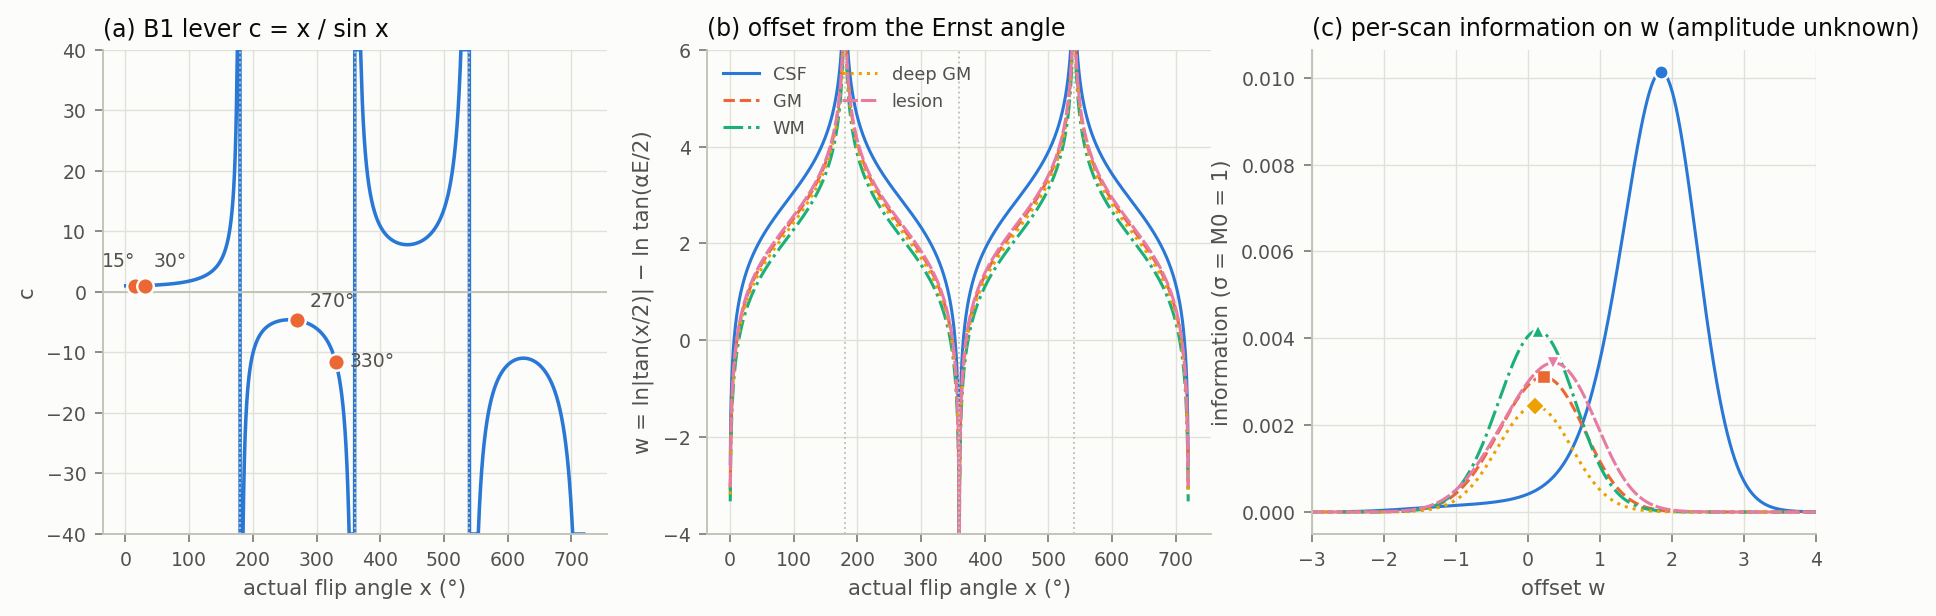
\includegraphics[width=\linewidth]{theory.png}
\caption{(a) The rate $c(x)=x/\sin x$ at which a sample moves along the log half-angle axis per unit
change of $\ln\Bone$. Dotted: multiples of $180^\circ$. (b) The offset \eqref{eq:w} of a sample
from each tissue's Ernst angle; $x$ and $360^\circ-x$ have the same offset. (c) Information about
$w$ in one scan with the amplitude unknown ($\Ttwo$, $\Ttwos$, $\dw$, $\phi_0$ known), against $w$; markers: maxima.}
\label{fig:theory}
\end{figure}

\Cref{tab:reduced} evaluates \cref{prop:closed,prop:ratio} for the shortlisted designs of
\cref{sec:constraints}; the closed forms agree with direct inversion of the $3\times3$ and $7\times7$
information to rounding. Freeing $\Ttwo$, $\Ttwos$, $\dw$ and $\phi_0$ costs $7$--$30\%$ in the $\Tone$ bound; in
\eqref{eq:closed} this is the information about the offsets that scan 2 must spend on $\Ttwo$ and $\Ttwos$.

\begin{table}[!htbp]
\centering
\caption{\Cref{prop:closed,prop:ratio} for the shortlist, WM at $\Bone=1$ (bounds per unit $\sigma/\Mzero$).
``known'': $\Ttwo$, $\Ttwos$, $\dw$, $\phi_0$ known; ``free'': all seven parameters free. Ratio bias: $\mathrm d\ln\Tone/\mathrm d\varepsilon$
and $\mathrm d\ln\Mzero/\mathrm d\varepsilon$. Last column: largest relative difference between the closed forms and direct
inversion of the $3\times3$ and $7\times7$ information. For $28^\circ/180^\circ$, $x_2=180^\circ$ at $\Bone=1$ and the closed form is a limit.}
\label{tab:reduced}
\small\setlength{\tabcolsep}{4pt}
\begin{tabular}{ccccccccc}
\toprule
& & \multicolumn{2}{c}{SD$(\ln\Bone)$} & \multicolumn{2}{c}{SD$(\ln\Tone)$} & \multicolumn{2}{c}{ratio bias} & closed vs\\
\cmidrule(lr){3-4}\cmidrule(lr){5-6}\cmidrule(lr){7-8}
$\alpha_1/\alpha_2$ & $L$ & known & free & known & free & $\Tone$ & $\Mzero$ & matrix\\
\midrule
15/330 & $-12.53$ & 2.16 & 2.21 & 25.5 & 27.3 & $-1.86$ & $-0.93$ & $1\times10^{-15}$\\
20/276 & $-5.86$ & 3.81 & 6.23 & 26.7 & 32.7 & $-1.69$ & $-0.84$ & $1\times10^{-15}$\\
14/309 & $-7.95$ & 3.27 & 5.09 & 25.7 & 30.3 & $-1.76$ & $-0.88$ & $4\times10^{-16}$\\
21/270 & $-5.74$ & 3.94 & 6.25 & 27.5 & 33.4 & $-1.68$ & $-0.84$ & $2\times10^{-15}$\\
17/254 & $-5.63$ & 4.47 & 8.33 & 25.2 & 32.6 & $-1.66$ & $-0.83$ & $1\times10^{-15}$\\
28/180 & $\infty$ & 7.00 & 7.00 & 44.6 & 53.0 & $-2.08$ & $-1.04$ & (limit)\\

\bottomrule
\end{tabular}
\end{table}

\section{The local design maps}\label{sec:maps}

\Cref{fig:maps} shows the worst-case and mean $\Tone$ bounds and the worst-case $\Bone$ bound over all
pairs with $\alpha_1\le90^\circ$. Pairs with $\alpha_1>90^\circ$ are never competitive: their best worst-case $\Tone$
bound is $1499$, fifteen times the optimum. Designs with a complex alias in the fitting range
(\cref{sec:aliases}) are greyed out; contours mark $1.05$ and $1.1$ times the best value among the
remaining designs.

\begin{figure}[!htbp]
\centering
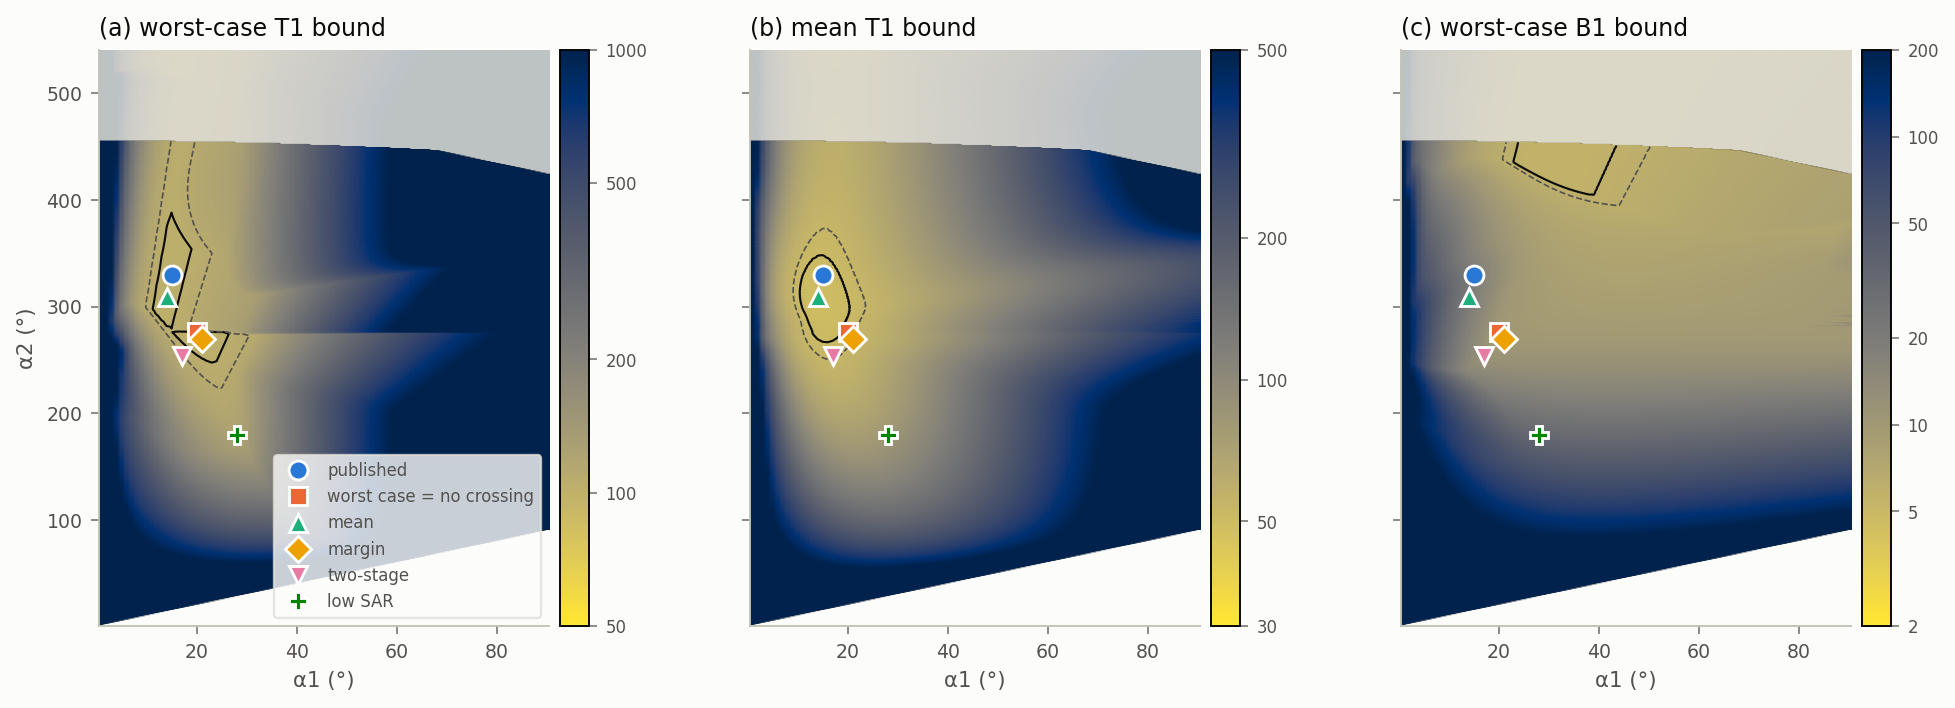
\includegraphics[width=\linewidth]{maps.png}
\caption{Design maps over the nominal angles ($1^\circ$ grid; bounds per unit $\sigma/\Mzero$, all parameters free).
(a) Worst case of the $\Tone$ bound over $\Bone\in[0.7,1.3]$ and the five tissues; (b) its mean; (c) worst
case of the $\Bone$ bound. Grey: a complex alias in the fitting range $[0.6,1.4]$. Solid and dashed
contours: $1.05$ and $1.1$ times the best value among designs without a complex alias. Markers: the
shortlist of \cref{tab:shortlist}.}
\label{fig:maps}
\end{figure}

\paragraph{The optimum is flat, and the published design is in it.} The best mean $\Tone$ bound,
$49.2$, is reached at $14^\circ/309^\circ$ (flat to $0.2\%$ for $\alpha_2=305$--$312^\circ$; the mean is an average over the
$0.01$ grid of $\Bone$); the published $15^\circ/330^\circ$ gives $50.2$, $2\%$ more. The designs within $5\%$ of the
optimum form a curved band (solid contour in \cref{fig:maps}b) that extends over $\alpha_1=11$--$20^\circ$
and $\alpha_2=267$--$348^\circ$: at $\alpha_1=15^\circ$ every $\alpha_2$ from $267^\circ$ to $348^\circ$ qualifies, at $11^\circ$ only $299$--$329^\circ$ and
at $20^\circ$ only $291$--$309^\circ$. The best worst-case bound, $100.3$, is reached at $20^\circ/276^\circ$; the published
design gives $103.6$, $3.3\%$ more. In terms of $\Tone$ precision alone, the flip angles of the
published protocol cannot be improved materially. The best $\alpha_1$ follows from \cref{fig:theory}c:
the information about the offset peaks at actual angles of $13$--$16^\circ$ for the parenchymal tissues,
just above their Ernst angles, and the lever of a near-$360^\circ$ pulse does the rest.

\paragraph{The worst case is decided by a narrow band.} The worst case of every near-$360^\circ$ design
is set by CSF where $\Bone\alpha_2=360^\circ$ (below). Outside a band of $\pm0.5\%$ in $\Bone$ around that crossing, the
published design's worst case is $91.9$ and the best design ($12^\circ/332^\circ$) reaches $89$; $20^\circ/276^\circ$ wins only
because its crossing lies just outside the range, at $\Bone=1.304$. Its $\alpha_2$ is therefore set by the
assumed upper limit of $\Bone$ ($\alpha_2=\lfloor360^\circ/1.3\rfloor$): the worst case jumps from $100.3$ at $\alpha_2=276^\circ$ to
$113.4$ at $277^\circ$. For parenchyma alone (no CSF) the best worst case is $61.0$ at $15^\circ/308^\circ$, against
$68.0$ for the published design ($-10\%$).

\paragraph{What the angles do decide.} Within the flat region the designs differ in the
secondary quantities. \Cref{fig:profiles} shows the bounds against $\Bone$ for the shortlist.
\begin{itemize}
\item \emph{The $360^\circ$ crossing.} For $\alpha_2$ between $277^\circ$ and $514^\circ$ the scan-2 pulse passes through
  $360^\circ$ somewhere in $\Bone\in[0.7,1.3]$ (at $\Bone=1.09$ for $330^\circ$). There the scan-2 signal vanishes and
  scan 2 measures only $\Bone$ (\cref{prop:closed}): the $\Bone$ bound has a deep minimum, and the $\Tone$ bound
  rises to that of scan 1 alone with $\Bone$ known. The rise comes from the loss of scan 2's
  information about $\Ttwo$ and $\Ttwos$; with these known there is no peak, and at $180^\circ$ crossings there
  is none either. The peak is about $0.5\%$ wide in $\Bone$ for CSF and $1$--$1.3\%$ for the parenchymal tissues,
  and it sets the worst case of the published design (CSF, $103.6$ against a mean of $82.8$).
\item \emph{Equal offsets.} In tissues with a short $\Ttwo$ the $\Tone$ bound also rises where the two
  scans sample the same offset, $w_1=w_2$, i.e.\ $x_2=360^\circ\pm x_1$ ($\Bone=1.04$ and $1.14$ for $15^\circ/330^\circ$): there the
  pathway ratios of the two scans coincide and separate $\Ttwo$ from $\Tone$ less well (\cref{fig:profiles}a).
\item \emph{No crossing.} $20^\circ/276^\circ$ keeps both pulses away from multiples of $180^\circ$ over the whole range,
  with no headroom at the top ($359^\circ$ at $\Bone=1.3$, where its bound rises). Its worst-case $\Bone$ bound is
  $10.2$ against $19.2$, and its scan-2 pulse needs $30\%$ less energy at equal pulse duration ($16\%$ less,
  with a $16\%$ shorter pulse, at equal peak $\Bone$). It pays $5\%$ in the mean $\Tone$ bound, mostly in CSF
  ($91.3$ against $82.8$); only WM is slightly better ($36.8$ against $37.4$), while GM, deep GM and lesion
  lose $2$--$4\%$. The design with $2.5\%$ headroom at both ends, $21^\circ/270^\circ$ ($\Bone$ crossings at $0.667$ and
  $1.333$), has nearly the same worst case ($101.4$) and $\Bone$ bound ($10.2$); $18^\circ/270^\circ$ trades $1\%$ of worst
  case for a better mean ($51.8$ against $53.7$) and a scan-1 $\Tone$ bound within $0.2\%$ of the two-stage
  optimum ($109.9$ against $109.7$ at $\alpha_1=17^\circ$).
\end{itemize}

\begin{figure}[!htbp]
\centering
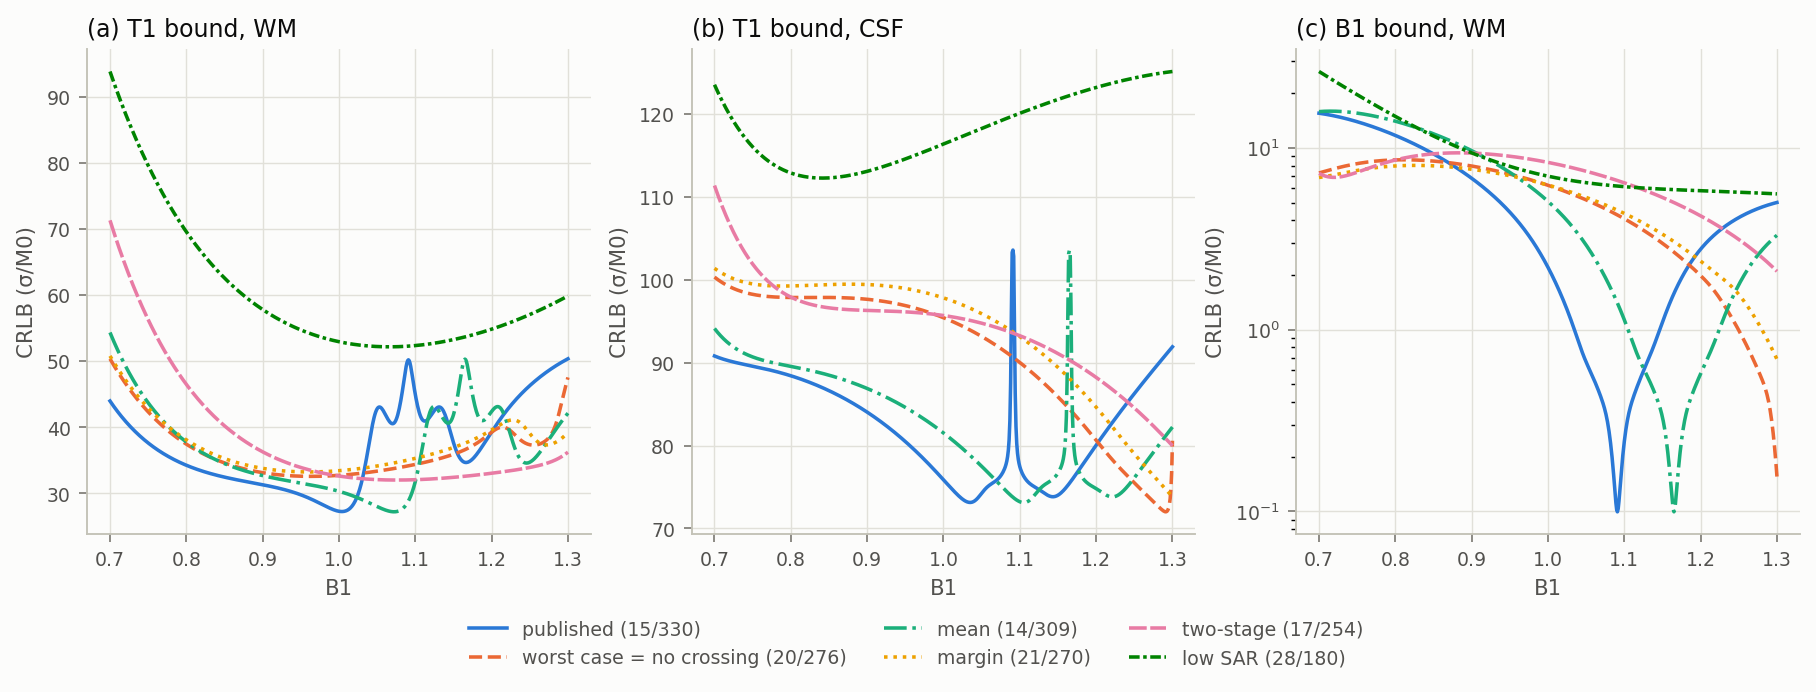
\includegraphics[width=\linewidth]{profiles.png}
\caption{Bounds against $\Bone$ for the shortlisted designs (all parameters free; the $\Bone$ grid
includes each design's crossing points). (a), (b) $\Tone$ bound for WM and CSF: the near-$360^\circ$ designs
show a narrow peak where $\Bone\alpha_2=360^\circ$, and in WM broader bumps where $w_1=w_2$. (c) $\Bone$ bound for
WM, logarithmic: the same crossing gives a null measurement of $\Bone$.}
\label{fig:profiles}
\end{figure}

\section{Global identifiability: aliases}\label{sec:aliases}

The bounds of \cref{sec:maps} are local. A design can have small bounds and still be unusable
if a different set of parameters reproduces the data exactly.

\begin{definition}[Alias]\label{def:alias}
For true parameters $\theta=(\Mzero,\Bone,\Tone,\Ttwo,\Ttwos,\dw,\phi_0)$, an \emph{alias} is a parameter vector
$\theta'=(\Mzero',B_1^{+\prime},\Tone',\Ttwo,\Ttwos,\dw,\phi_0')$ with $B_1^{+\prime}\ne\Bone$ and a physical $\Tone'$ (an Ernst angle in
$(0^\circ,90^\circ)$, i.e.\ $0<\tan(\alpha_E'/2)<1$) whose noise-free signals equal those of $\theta$ in every
pathway, echo and scan. It is a \emph{complex alias} if the complex signals agree (with $\phi_0'=\phi_0+\pi$
allowed, which absorbs a sign change of both scans), and a \emph{magnitude alias} if only their
magnitudes do.
\end{definition}

$\Ttwo$, $\Ttwos$ and $\dw$ are held at their true values because the echo decay and the echo phases
determine them (up to phase wraps of $\dw$); the characterisation below also uses that the pattern
of pathway amplitudes determines $u$, which holds numerically for the tissues considered.

An alias is not a nearby value and not a poorly determined one: the least-squares cost has an
equally deep minimum at $\theta'$, and for noisy data every minimum near the truth has a twin near
$\theta'$ with identical cost. No signal-to-noise ratio separates them; only prior knowledge (a
fitting range for $\Bone$) or additional data can. This distinguishes an alias from a local minimum
(higher cost, avoidable with better starting values) and from poor conditioning (a unique but
noisy solution).

\paragraph{Where aliases come from.} Two scans determine $w_1$, $w_2$ and $\ell$; complex data with a
phase shared by the two scans also determine the relative sign of $v_1$ and $v_2$. Dividing the two
half-angle ratios $\xi_i=\tan(x_i/2)/\zeta$ eliminates $\Tone$ and $\Mzero$ and leaves one equation in $\Bone$ alone,
\begin{equation}
  f(\Bone)=\frac{\tan(\Bone\alpha_2/2)}{\tan(\Bone\alpha_1/2)}=\frac{\xi_2}{\xi_1},
  \label{eq:f}
\end{equation}
whose right side the data fix (\cref{fig:alias}). Every other root $B_1^{+\prime}$ of \eqref{eq:f} with
\[
  \tan(\alpha_E'/2)=\zeta\,\Bigl|\frac{\tan(B_1^{+\prime}\alpha_1/2)}{\tan(\Bone\alpha_1/2)}\Bigr|<1
\]
is a complex alias, with $\Mzero'=\Mzero\zeta/\tan(\alpha_E'/2)$; every admissible root of $f(B_1^{+\prime})=-f(\Bone)$ is a
magnitude alias, in which the scan-2 signal is negated relative to scan 1. The alias values
of $\Bone$ depend on the true $\Bone$ alone, not on the tissue; the tissue enters only through $\Tone'$ and
through admissibility. For the published design and true $\Bone=1$ ($f=-2.04$) the magnitude alias
is $B_1^{+\prime}=1.199$ (the scan-2 pulse becomes $395.7^\circ\equiv+35.7^\circ$ instead of $330^\circ\equiv-30^\circ$; $\Tone'=588$\,ms
for WM) and the complex alias is $B_1^{+\prime}=2.008$ ($\Tone'=203$\,ms), excluded by any fitting range below
$\Bone=540/330$; more generally, a fitting range inside $(180^\circ/\alpha_2,540^\circ/\alpha_2)=(0.545,1.636)$
excludes every complex alias for true $\Bone$ in it, because $f$ is monotonic on that branch.

\paragraph{Local and global identifiability are linked.} Differentiating \eqref{eq:f},
\begin{equation}
  \frac{\mathrm d\ln|f|}{\mathrm d\ln\Bone}=c(\Bone\alpha_2)-c(\Bone\alpha_1)=L ,
  \label{eq:dlnf}
\end{equation}
the lever of \cref{prop:closed}. Since $f'=f\,L/\Bone$, $f$ is monotonic on an interval between consecutive
poles ($x_2=180^\circ+360^\circ m$ or $x_1=360^\circ m$) exactly where $f\,L$ keeps its sign; $L$ itself changes sign only
at the zeros of $f$, where $f'$ stays finite. A complex alias on the same branch therefore requires a
point with $L=0$, where the information is singular. Magnitude aliases arise around each zero of $f$ ($x_2=360^\circ m$ or $x_1=180^\circ+360^\circ m$) and each
pole ($x_2=180^\circ+360^\circ m$) inside the fitting range, where $f$ changes sign.

\begin{proposition}[No aliases without crossings]\label{prop:noalias}
If over the whole fitting range $x_1=\Bone\alpha_1\in(0^\circ,180^\circ)$ and $x_2=\Bone\alpha_2\in(180^\circ,360^\circ)$, the design has no
alias of either kind in that range.
\end{proposition}
\begin{proof}
There $\tan(x_1/2)>0>\tan(x_2/2)$, so $f<0$, and $c_1>0>c_2$, so $L<0$; by \eqref{eq:dlnf} $|f|$ is strictly
decreasing, hence one-to-one, and $f(B_1^{+\prime})=\pm f(\Bone)$ has no root other than $\Bone$.
\end{proof}

\begin{figure}[!htbp]
\centering
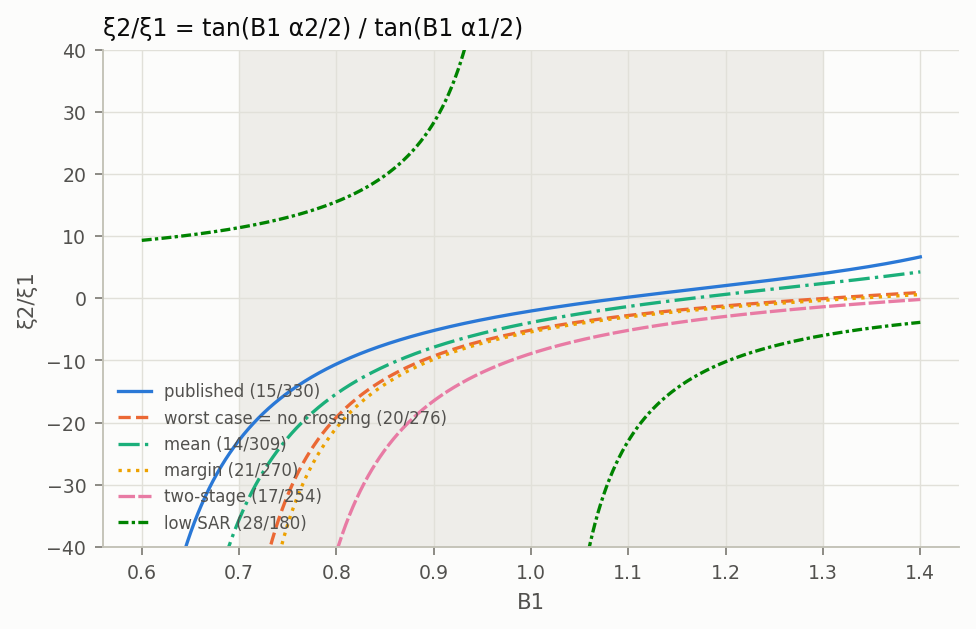
\includegraphics[width=0.75\linewidth]{alias.png}
\caption{The $\Bone$-only quantity \eqref{eq:f} for the shortlist over the fitting range $[0.6,1.4]$
(shaded: robustness range). A complex alias exists if a horizontal line meets a curve twice
within the fitting range; a magnitude alias if it meets the curve and its mirror image $-f$.}
\label{fig:alias}
\end{figure}

\paragraph{Aliases over the design space.} With the fitting range $[0.6,1.4]$, of the 145\,530 pairs
\AliasComplex{} have a complex alias for some true $\Bone$ in $[0.7,1.3]$ (mostly pairs with a large $\alpha_1$ or
an $\alpha_2$ above about $450^\circ$, greyed in \cref{fig:maps}), \AliasMagnitude{} have only magnitude aliases and
\AliasNone{} have none. This fitting range spans a factor $2.3$ in $\Bone$, more than any pulse can stay
within $(180^\circ,360^\circ)$, so every near-optimal design has a magnitude alias somewhere in it: the best
design without any alias has a worst-case $\Tone$ bound of $197$, twice the optimum. With $[0.6,1.4]$ a
good protocol therefore needs complex data, or for magnitudes the one bit of phase supplied by
the FID-sign test~\cite{technote}. A narrower fitting range changes this for the no-crossing designs:
fitted within their own crossing-free range (e.g.\ $\Bone\in[0.667,1.333]$ for $\alpha_2=270^\circ$, which still
contains the robustness range), they have no alias at all (\cref{prop:noalias}), and magnitude-only
fitting becomes possible. All shortlisted designs are free of complex aliases on $[0.6,1.4]$;
\cref{tab:shortlist} lists where their magnitude aliases occur. For the published design they
cover most of the range (true $\Bone\ge0.87$); for the no-crossing designs only its ends, near the
crossings that lie just outside it, with the alias $1$--$16\%$ from the truth and near the edge of the
fitting range.

\section{Constraints and shortlist}\label{sec:constraints}

\paragraph{SAR and peak $\Bone$.} \Cref{fig:pareto}a gives the best joint design (no complex alias)
as a function of the largest nominal angle. Both curves are flat above about $280^\circ$ (worst case)
and $310^\circ$ (mean): larger pulses buy nothing. Below, the price rises steadily. A limit of $240^\circ$
costs $6\%$ in the worst case and $14\%$ in the mean; a limit of $180^\circ$ costs $25\%$ and $52\%$; a
limit of $120^\circ$ more than doubles both. Relative to $330^\circ$, a second pulse at $276^\circ$ needs $30\%$ less
energy at equal pulse duration; at equal peak $\Bone$ it is $16\%$ shorter and needs $16\%$ less energy.

\paragraph{Two-stage pipeline.} When scan 2 serves only to map a smooth $\Bone$, $\alpha_1$ should minimise
the scan-1 $\Tone$ bound with $\Bone$ known (\cref{fig:pareto}b). The minimum lies at $17^\circ$ (worst case,
$109.7$) to $19^\circ$ (mean, $64.5$), against $117.8$ and $68.0$ at $15^\circ$: a gain of $5$--$7\%$, consistent with
the information peak just above the Ernst angles (\cref{fig:theory}c). Between $15^\circ$ and $22^\circ$ the worst case
varies by about $7\%$. Because smoothing makes the noise in the $\Bone$ map negligible~\cite{technote}, $\alpha_2$ is
chosen for an alias-free, well-conditioned $\Bone$ measurement and for robustness; restricted to
$\alpha_2\le330^\circ$ (no more SAR than the published design), the smallest worst-case $\Bone$ bound for
$\alpha_1=17^\circ$ is at $\alpha_2=254^\circ$ (without the restriction it lies near $440^\circ$, a larger lever at $78\%$ more
energy, \cref{fig:maps}c). This pulse crosses $180^\circ$ at $\Bone=0.71$, which costs nothing in the $\Tone$ bound but
produces magnitude aliases for $\Bone$ below $0.8$; $\alpha_2=258$--$270^\circ$ avoids the crossing (e.g.\ $17^\circ/270^\circ$:
worst-case $\Bone$ bound $12.3$ against $11.2$).

\begin{figure}[!htbp]
\centering
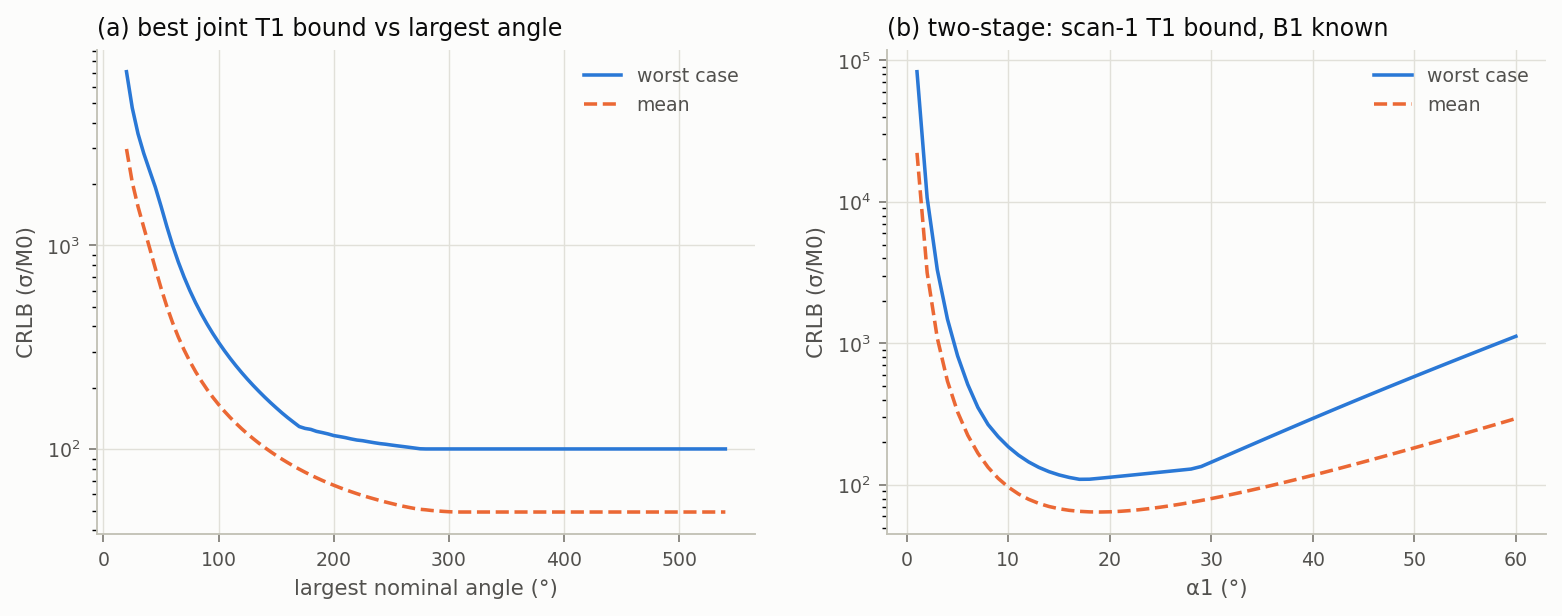
\includegraphics[width=\linewidth]{pareto.png}
\caption{(a) Best worst-case and mean joint $\Tone$ bound among designs without a complex alias whose
largest angle does not exceed the abscissa. (b) Two-stage pipeline: scan-1 $\Tone$ bound with $\Bone$ known
against $\alpha_1$ (worst case and mean over $\Bone\in[0.7,1.3]$ and the tissues).}
\label{fig:pareto}
\end{figure}

\paragraph{Shortlist.} \Cref{tab:shortlist} collects the designs carried forward. The rules that
select them are: the published design; the minimum worst-case and minimum mean joint $\Tone$
bound; the best design whose pulses cross no multiple of $180^\circ$ for $\Bone\in[0.7,1.3]$ (it coincides
with the worst-case optimum, $\alpha_2=258$--$276^\circ$); the best such design with $2.5\%$ headroom at both ends
of the range (\emph{margin}, $\alpha_2=264$--$270^\circ$); the two-stage design above; and the best design with
both angles at most $180^\circ$. All are free of complex aliases in the fitting range; the last column
gives the true $\Bone$ for which a magnitude alias exists.

\begin{table}[!htbp]
\centering
\caption{Shortlisted designs. Bounds per unit $\sigma/\Mzero$, all parameters free, worst case (w.) or
mean over $\Bone\in[0.7,1.3]$ and the five tissues; ``par.'': parenchyma only (no CSF). Scan-1 $\Tone$:
two-stage criterion ($\Bone$ known). Ratio bias: largest $|\mathrm d\ln\Tone/\mathrm d\varepsilon|$ over the range. Last column:
true $\Bone$ with a magnitude alias in the fitting range $[0.6,1.4]$ (no design has a complex alias).}
\label{tab:shortlist}
\footnotesize\setlength{\tabcolsep}{3pt}
\begin{tabular}{lccccccccc}
\toprule
& & \multicolumn{3}{c}{$\Tone$ bound} & $\Bone$ & $\Ttwo$ & scan-1 $\Tone$ & ratio & \\
\cmidrule(lr){3-5}
Design & $\alpha_1/\alpha_2$ & w. & mean & w.\ par. & w. & w. & w., $\Bone$ known & bias & magn.\ alias\\
\midrule
published & 15/330 & 103.6 & 50.2 & 68.0 & 19.2 & 117.3 & 117.8 & 2.34 & 0.87--1.30\\
worst case = no crossing & 20/276 & 100.3 & 52.6 & 73.9 & 10.2 & 115.9 & 113.4 & 2.06 & 1.22--1.30\\
mean & 14/309 & 103.6 & 49.2 & 61.9 & 20.5 & 130.1 & 124.3 & 2.25 & 0.99--1.30\\
margin & 21/270 & 101.4 & 53.7 & 63.7 & 10.2 & 114.8 & 115.3 & 2.02 & 0.70--0.72, 1.27--1.30\\
two-stage & 17/254 & 111.4 & 53.6 & 78.5 & 11.2 & 124.0 & 109.7 & 2.04 & 0.70--0.79\\
low SAR & 28/180 & 125.1 & 81.9 & 117.0 & 32.0 & 127.6 & 129.7 & 3.26 & 0.70--1.00, 1.00--1.21\\

\bottomrule
\end{tabular}
\end{table}

\section{Robustness to model error}\label{sec:robustness}

The bounds assume that the fitting model is exact. \Cref{tab:robustness} generates noise-free
data with an effect the ideal model ignores and fits them with the ideal two-scan model (complex,
all seven parameters free, ten starting points, $\Bone$ restricted to the fitting range $[0.6,1.4]$) for
WM, GM and CSF at $\Bone=0.7,0.8,\dots,1.3$ and at the transmit scales where the design's scan-2 angle is
$330^\circ$ and $345^\circ$.
\begin{itemize}
\item \emph{Pulse ratio}: the scan-2 angle $1\%$ larger than nominal relative to scan 1, as produced
  by an imperfect calibration of two pulses of different shape or duration.
\item \emph{Slab-edge ramp}: the flip angle falls linearly from $100\%$ to $90\%$ across the voxel, each
  position in its own steady state, as at the edge of a 3D slab.
\item \emph{Finite pulses}: hard pulses at a fixed peak $\Bone$, so that the duration is proportional to
  the nominal angle ($1$\,ms for $330^\circ$), with relaxation during the pulse; echo times are measured
  from the pulse centre. On resonance, and with $50$\,Hz off resonance (precession during the pulse).
\end{itemize}
Besides the bias we give the probability that the misfit would be flagged at SNR 300 by a $\chi^2$
test on the residual (level $99.9\%$, 29 degrees of freedom; noncentral $\chi^2$ with the noise-free
residual as noncentrality).

\begin{table}[!htbp]
\centering
\caption{Bias of $\Tone$, $100(\hat\Tone/\Tone-1)$ (\%), when the ideal two-scan model is fitted to data with
the effect (noise-free, all parameters free). Columns 3--5: at $\Bone=1$; column 6: largest $|$bias$|$ over
WM, GM, CSF and the sampled $\Bone$ ($0.7,0.8,\dots,1.3$ and the scan-2 angles $330^\circ$, $345^\circ$), a lower bound
for the continuous range; column 7: largest $|\delta\ln\Tone|$ divided by the $\Tone$
standard deviation at SNR$(\Mzero)=300$ (bound/300); column 8: probability that the misfit of the
largest-bias case is flagged at SNR 300. $^*$: a fit ended on a safeguard bound of the optimiser.
Generated by \texttt{scripts/flip\_design\_robustness.py}.}
\label{tab:robustness}
\small\setlength{\tabcolsep}{4pt}
\begin{tabular}{llcccccc}
\toprule
& & \multicolumn{3}{c}{$\Bone=1$} & \multicolumn{3}{c}{largest over the sampled cases}\\
\cmidrule(lr){3-5}\cmidrule(lr){6-8}
$\alpha_1/\alpha_2$ & effect & WM & GM & CSF & $|$bias$|$ (\%) & $|$bias$|$/SD & flagged\\
\midrule
15/330 & pulse ratio $+1\%$ & $-1.8$ & $-1.8$ & $-1.8$ & 2.3 & 0.2 & 0.00\\
 & slab-edge ramp & $+1.7$ & $+0.9$ & $+0.7$ & 40.3 & 1.3 & 0.58\\
 & finite pulses & $+19.7$ & $+18.5$ & $+5.4$ & 19.7 & 2.0 & 0.04\\
 & finite pulses, 50\,Hz & $+22.2$ & $+19.6$ & $+11.9$ & 22.2 & 2.2 & 0.99\\
\midrule
20/276 & pulse ratio $+1\%$ & $-1.7$ & $-1.7$ & $-1.7$ & 2.1 & 0.2 & 0.00\\
 & slab-edge ramp & $-0.3$ & $-0.3$ & $-0.2$ & 16.3 & 1.1 & 0.10\\
 & finite pulses & $+2.4$ & $+2.2$ & $+0.6$ & 13.8 & 1.2 & 0.01\\
 & finite pulses, 50\,Hz & $+2.7$ & $+2.5$ & $+3.8$ & 13.3 & 1.1 & 0.92\\
\midrule
14/309 & pulse ratio $+1\%$ & $-1.8$ & $-1.8$ & $-1.8$ & 2.2 & 0.2 & 0.00\\
 & slab-edge ramp$^*$ & $-0.1$ & $-0.3$ & $0.0$ & 74.1 & 3.9 & 0.83\\
 & finite pulses & $+6.4$ & $+5.1$ & $+0.6$ & 19.5 & 2.0 & 0.03\\
 & finite pulses, 50\,Hz & $+6.9$ & $+5.6$ & $+8.4$ & 21.9 & 2.2 & 0.98\\
\midrule
21/270 & pulse ratio $+1\%$ & $-1.7$ & $-1.7$ & $-1.7$ & 2.0 & 0.2 & 0.00\\
 & slab-edge ramp & $-0.3$ & $-0.3$ & $-0.1$ & 13.0 & 0.8 & 0.02\\
 & finite pulses & $+2.2$ & $+2.1$ & $+1.8$ & 14.4 & 1.2 & 0.01\\
 & finite pulses, 50\,Hz & $+2.5$ & $+2.4$ & $+3.5$ & 13.9 & 1.2 & 0.88\\
\midrule
17/254 & pulse ratio $+1\%$ & $-1.6$ & $-1.6$ & $-1.6$ & 2.0 & 0.2 & 0.00\\
 & slab-edge ramp & $-0.2$ & $-0.2$ & $0.0$ & 0.9 & 0.1 & 0.00\\
 & finite pulses & $+2.0$ & $+1.9$ & $+2.1$ & 10.0 & 0.8 & 0.05\\
 & finite pulses, 50\,Hz & $+2.3$ & $+2.2$ & $+3.1$ & 11.1 & 0.9 & 0.88\\
\midrule
28/180 & pulse ratio $+1\%$ & $-2.0$ & $-2.0$ & $-2.0$ & 3.1 & 0.1 & 0.00\\
 & slab-edge ramp & $-0.2$ & $-0.2$ & $0.0$ & 0.4 & 0.0 & 0.00\\
 & finite pulses & $+2.0$ & $+2.0$ & $+1.8$ & 3.4 & 0.1 & 0.00\\
 & finite pulses, 50\,Hz & $+2.3$ & $+2.3$ & $+2.2$ & 4.0 & 0.1 & 0.00\\

\bottomrule
\end{tabular}
\end{table}

\paragraph{Pulse ratio: the same for every design, and invisible.} A $1\%$ ratio error biases $\Tone$ by
$-1.6$ to $-2.0\%$ at $\Bone=1$ in every design (up to $-3.1\%$ over the $\Bone$ range), as \cref{prop:ratio}
predicts, and the fit absorbs it with zero residual. No choice of angles avoids it
($|\mathrm d\ln\Tone/\mathrm d\varepsilon|\ge1.64$): the ratio must be calibrated, to about $0.5\%$ if $\Tone$ is to be accurate to
$1\%$. The bias is only $0.2$ standard deviations per voxel at SNR 300, but it is systematic and does
not average out over a region.

\paragraph{Everything goes wrong near $360^\circ$.} The other two effects share one pattern: they bias
$\Tone$ strongly where the actual scan-2 angle approaches $360^\circ$, i.e.\ where its effective angle is small
(finite pulses most at $330$--$350^\circ$, flip-angle spreads at and across $360^\circ$), and hardly at all elsewhere; crossings of $180^\circ$ are harmless, because the scan-2 signal there is
small in any case ($|v|\approx\zeta^2|\delta|$ at $180^\circ+\delta$ against $|\delta|$ at $360^\circ+\delta$).
\begin{itemize}
\item \emph{Finite pulses.} With a $1$\,ms $330^\circ$ pulse the published design overestimates $\Tone$ by $20\%$
  in WM and $18.5\%$ in GM at $\Bone=1$, two standard deviations at SNR 300, with a misfit that is flagged
  in only $2$--$4\%$ of voxels. The margin design $21^\circ/270^\circ$ gives $2.2\%$ and $2.1\%$ there. The bias grows with
  the pulse duration: for a $330^\circ$ pulse of $0.125$, $0.25$, $0.5$, $1$, $2$ and $4$\,ms it is $3.4$, $6.6$, $12.7$,
  $19.7$, $22.6$ and $33.6\%$ for the published design (steep, then irregular) and $0.27$, $0.54$, $1.1$, $2.2$,
  $4.5$ and $9.6\%$ for $21^\circ/270^\circ$ (nearly proportional; durations scale with the nominal angle, so the
  $270^\circ$ pulse lasts $270/330$ of these). The advantage is local, though: every design meets the same
  problem where its scan-2 pulse passes $330$--$350^\circ$ (the margin design at $\Bone=1.28$, $-14\%$; $20^\circ/276^\circ$ at
  $\Bone=1.25$, $-14\%$; $17^\circ/254^\circ$ at $\Bone=1.3$, $+10\%$), so over the whole range the largest bias falls only from
  $20\%$ to $10$--$14\%$ for the no-crossing designs ($14^\circ/309^\circ$ reaches $19.5\%$ at its $330^\circ$ point; $3\%$ for the
  $180^\circ$ design, whose scan-2 pulse never gets there). Off resonance the
  misfit of the designs with $\alpha_2\ge254^\circ$ becomes detectable (flagged in $88$--$99\%$ of voxels in the
  worst case); the bias changes by at most $2.5$ points in WM and GM but grows in CSF (e.g.\ from
  $0.6$ to $8.4\%$ for $14^\circ/309^\circ$ at $\Bone=1$). Finite-pulse effects are deterministic and can be built into the
  forward model, as is done for balanced SSFP~\cite{bieri2009}; any design whose scan-2 pulse reaches
  $330$--$360^\circ$ over the $\Bone$ range needs it.
\item \emph{Slab-edge spread.} All designs estimate $\Bone$ as the voxel average ($\approx-5\%$) and $\Tone$ within
  $2\%$ as long as the scan-2 angle stays below about $330^\circ$. Near $360^\circ$ the bias grows: $-13\%$ and $-16\%$
  for $21^\circ/270^\circ$ and $20^\circ/276^\circ$ at $\Bone=1.3$ (scan-2 angle $351^\circ$ and $359^\circ$), and $+32$ to $+74\%$ where the
  spread straddles $360^\circ$ (the published design at $\Bone=1.1$--$1.2$, $14^\circ/309^\circ$ at $1.2$), because the two sides of
  the null contribute signals of opposite sign. These misfits are hard to detect: the $40\%$ CSF
  bias of the published design at $\Bone=1.2$ is flagged in $58\%$ of voxels, the $16\%$ bias of $20^\circ/276^\circ$ in
  $10\%$, and the margin design's $13\%$ in $2\%$. The two-stage design $17^\circ/254^\circ$, whose scan-2 angle never
  exceeds $330^\circ$, stays below $1\%$.
\end{itemize}

\paragraph{2D slice profiles.} An unmodelled 2D slice profile is a much larger error than the
slab-edge spread and is not tabulated: the scaled small-tip profile used for the slab edge is not
valid for a $250$--$330^\circ$ sinc pulse, whose rotation axis and tip angle vary across the slice in a
way only a Bloch simulation of the pulse captures. MPME relaxometry needs a 3D acquisition, as
in~\cite{cheng2019}, or the slice profile in the forward model.

\section{Recommendations and limitations}\label{sec:recommendations}

\paragraph{Recommendations.}
\begin{enumerate}
\item \emph{Do not expect precision gains from the flip angles alone.} For the joint fit the
  published $15^\circ/330^\circ$ is within $2\%$ (mean) and $3.3\%$ (worst case) of the best $\Tone$ bound, inside a
  broad band of near-optimal designs (\cref{sec:maps}).
\item \emph{Keep the scan-2 pulse away from $360^\circ$ over the whole $\Bone$ range.} Near $360^\circ$ the $\Tone$ bound
  peaks (CSF), magnitude aliases come close to the truth, and unmodelled finite pulses
  ($10$--$20\%$) and flip-angle spreads ($13$--$75\%$) bias $\Tone$, often without a detectable misfit on
  resonance. Crossings of $180^\circ$ are
  harmless. For $\Bone\in[0.7,1.3]$ this means $\alpha_2$ below $360^\circ/1.3=277^\circ$, and preferably with headroom:
  \begin{itemize}
  \item $\alpha_2\approx270^\circ$ (e.g.\ $21^\circ/270^\circ$ or $18^\circ/270^\circ$): worst-case $\Tone$ bound within $1$--$2.5\%$ of the optimum,
    worst-case $\Bone$ bound $10$--$11$ against $19$, $33\%$ less energy at equal pulse duration than $330^\circ$, and
    no aliases of any kind when fitted with $\Bone\in[0.667,1.333]$ (\cref{prop:noalias}), so magnitude
    data suffice. It pays $3\%$ ($18^\circ/270^\circ$, all in CSF; it matches the published design in every
    parenchymal tissue) to $7\%$ ($21^\circ/270^\circ$, about $60\%$ in CSF, with $4$--$7\%$ in GM and deep GM) in the
    mean $\Tone$ bound;
  \item $\alpha_2\approx255^\circ$ (e.g.\ $17^\circ/254^\circ$): the scan-2 angle stays below $330^\circ$ over the range, so the
    slab-edge spread costs $<1\%$; it crosses $180^\circ$ near $\Bone=0.71$ (harmless for $\Tone$, magnitude aliases
    below $\Bone=0.8$) and pays about $7\%$ in both $\Tone$ criteria relative to the published design.
  \end{itemize}
\item \emph{Model the finite pulse duration} whatever the design: unmodelled, pulses at the peak $\Bone$ of a
  $1$\,ms $330^\circ$ pulse bias $\Tone$ by $2$--$20\%$, most where the scan-2 angle passes $330$--$350^\circ$, which every
  design with $\alpha_2\ge254^\circ$ does somewhere in $[0.7,1.3]$.
\item \emph{Two-stage pipeline}: $\alpha_1=17$--$19^\circ$ ($5$--$7\%$ better than $15^\circ$ for the $\Tone$ step), with
  $\alpha_2\approx255$--$270^\circ$ for the $\Bone$ map.
\item \emph{Under a SAR limit}, $\alpha_{\max}=240^\circ$ costs $6$--$14\%$ and $180^\circ$ costs $25$--$52\%$ in the $\Tone$ bound;
  below about $150^\circ$ the precision falls off quickly (\cref{fig:pareto}a).
\item \emph{Calibrate the pulse ratio.} Every design transfers a ratio error to $\Tone$ with a factor of at
  least $1.64$ ($1.66$--$3.26$ over the $\Bone$ range in the shortlist), undetectably.
\item \emph{Fitting range and data type.} With a wide fitting range such as $[0.6,1.4]$ every good design
  has magnitude aliases, and complex data or the FID-sign test are needed; a no-crossing design
  fitted within its own crossing-free range has none.
\item \emph{Use a 3D acquisition} or model the slice profile.
\end{enumerate}

\paragraph{Limitations.} The criteria are local Cram\'er--Rao bounds under complex Gaussian
noise; they predict the precision of an efficient estimator (which joint maximum likelihood
attains for this model~\cite{technote}) but not its failure rate. The design space fixes $\TR$, the
readout and the time per scan; the robustness range weights $\Bone$ uniformly and the five tissues
equally, the worst case is dominated by CSF, and the worst-case optimum moves with the assumed
upper limit of $\Bone$. The model-error study is noise-free, uses one representative of each effect
and fits the two-stage design with the joint model rather than as a two-stage pipeline. Steps that
remain: Monte Carlo with the actual estimator for the shortlist (bias, efficiency, failure and alias
rates over the $\Bone$ range), phantom and BrainWeb simulations with a realistic $\Bone$ field, and a design
with the finite pulses in the forward model.


\appendix
\section{Computation and reproducibility}\label{app:repro}

\paragraph{Information.} Single-scan Jacobians come from the exact implicit-differentiation
Jacobian of the complex model (\texttt{mpme.fastjac}, 256 isochromats, float64), evaluated with a
$1^\circ$ nominal pulse and $\Bone=x$ so that the $\ln\Bone$ column is $\partial/\partial\ln x$
(\cref{prop:decomp}). Designs: all pairs $\alpha_1<\alpha_2$ on a $1^\circ$ grid in $[1^\circ,540^\circ]$ (145\,530
pairs); $\Bone$ on $[0.7,1.3]$ in steps of $0.01$, plus each pair's own crossing points
$\Bone=180^\circ k/\alpha_i$, where the bounds peak; five tissues. Bounds are $\sqrt{\operatorname{diag}\Fi^{-1}}$ of the
diagonally normalised matrix, rescaled. Runtime about $15$ minutes on a laptop CPU.

\paragraph{Aliases.} For every pair and every true $\Bone\in[0.7,1.3]$ (steps of $0.01$), the roots of
$f(b')-f(\Bone)$ (complex) and $|f(b')|-|f(\Bone)|$ (magnitude) on $b'\in[0.6,1.4]$ are bracketed on each
continuous branch of $f$ (4001-point grid) and kept if admissible for at least one tissue
($\zeta\,|\tan(b'\alpha_1/2)/\tan(\Bone\alpha_1/2)|<1$). The vectorised map agrees with the exact root finder
\texttt{mpme.design.alias\_roots} on spot checks, and the root finder reproduces the known aliases
of the published protocol at true $\Bone=1$: the magnitude alias $1.1991$ in $[0.6,1.4]$ and the complex alias
$2.0078$ in $[0.3,3]$.

\paragraph{Checks.} \Cref{prop:decomp} against direct evaluation of the two-scan information
(\texttt{mpme.crlb}): agreement to $3\times10^{-15}$ relative. \Cref{prop:perscan} ($J_{\Tone}=h(J_{\Bone}/c-J_{\Mzero})$):
$10^{-14}$ at angles from $15^\circ$ to $330^\circ$ and $\Tone$ from 600 to 4000\,ms. \Cref{prop:closed,prop:ratio}:
\cref{tab:reduced}. These are unit tests in \texttt{tests/test\_design.py} (tolerances $10^{-10}$, $10^{-12}$, $10^{-9}$ and $10^{-8}$
for the four checks).

\paragraph{Model-error fits.} Each fit of \cref{sec:robustness} starts from the truth and from nine
points ($\Bone\in\{0.75,1,1.25\}$, $\Tone\in\{0.5,1,2\}\times$ truth); the lowest cost with $\Bone$ in the fitting range is
kept, and fits ending on a safeguard bound of the optimiser are flagged.

\paragraph{Scripts.}
\begin{center}
\small
\begin{tabular}{ll}
\toprule
Result & Script\\
\midrule
Bounds, biases and alias status of all designs & \texttt{scripts/flip\_design.py}\\
Shortlist, \cref{fig:theory,fig:maps,fig:profiles,fig:pareto,fig:alias}, \cref{tab:reduced,tab:shortlist} &
  \texttt{scripts/flip\_design\_report.py}\\
Model-error biases, \cref{tab:robustness} & \texttt{scripts/flip\_design\_robustness.py}\\
\bottomrule
\end{tabular}
\end{center}
All are run by \texttt{make flipnote}. The design functions are in \texttt{src/mpme/design.py}.


\begin{thebibliography}{9}
\bibitem{cheng2019} C.-C.~Cheng, F.~Preiswerk, W.~S.~Hoge, T.-H.~Kuo, B.~Madore.
  Multipathway multi-echo (MPME) imaging: all main MR parameters mapped based on a single
  3D scan. \emph{Magn.\ Reson.\ Med.} 81(3):1699--1713, 2019.
\bibitem{technote} S.~Joshi. Multi-pathway multi-echo (MPME) relaxometry: forward model,
  information limits, and efficient estimation. Technical note, \texttt{docs/technote} of this
  repository.
\bibitem{deoni2003} S.~C.~L.~Deoni, B.~K.~Rutt, T.~M.~Peters. Rapid combined $T_1$ and $T_2$
  mapping using gradient recalled acquisition in the steady state. \emph{Magn.\ Reson.\ Med.}
  49(3):515--526, 2003.
\bibitem{yarnykh2007} V.~L.~Yarnykh. Actual flip-angle imaging in the pulsed steady state: a
  method for rapid three-dimensional mapping of the transmitted radiofrequency field.
  \emph{Magn.\ Reson.\ Med.} 57(1):192--200, 2007.
\bibitem{bieri2009} O.~Bieri, K.~Scheffler. SSFP signal with finite RF pulses.
  \emph{Magn.\ Reson.\ Med.} 62(5):1232--1241, 2009.
\end{thebibliography}

\end{document}
